
\documentclass[10pt, onecolumn]{scrartcl}
\usepackage{amsmath, graphicx}
\usepackage{xcolor}
\usepackage[top=1in, bottom=1in, left=1in, right=1in, includefoot]{geometry}
\usepackage{fancyvrb}
\usepackage{siunitx}
\usepackage[formats]{listings}
\usepackage[unicode=true]{hyperref}
\usepackage{enumitem}


\lstdefinelanguage{ucf}{
  sensitive=false,
  alsoletter={.},
  morekeywords={NET,LOC},
  morecomment=[l]{\#},
  morestring=[b]"
}


\lstdefineformat{Vlog}{~=\( \sim \),^=\(^\wedge\)}

\lstset{ %
  basicstyle=\ttfamily,        % the size of the fonts that are used for the code
  	format=Vlog,
  breaklines=false,                 % sets automatic line breaking
  language=Verilog,
  commentstyle=\color{red},    % comment style
  frame=single,                    % adds a frame around the code
  keepspaces=true,                 % keeps spaces in text, useful for keeping indentation of code (possibly needs columns=flexible)
  keywordstyle=\color{blue},       % keyword style
  morekeywords={*,...},            % if you want to add more keywords to the set
  rulecolor=\color{black},         % if not set, the frame-color may be changed on line-breaks within not-black text (e.g. comments (green here))
  showspaces=false,                % show spaces everywhere adding particular underscores; it overrides 'showstringspaces'
  tabsize=7,                       % sets default tabsize to 2 spaces
}

\usepackage{tikz}
\usepackage[american]{circuitikz}
\usetikzlibrary{calc,positioning,arrows,shapes.geometric}

\tikzset{
  multiplexer/.style={
    draw,
    trapezium,
    shape border uses incircle, 
    shape border rotate=270,
    minimum size=18pt
  }  
}


\ctikzset{bipoles/not port/circle width=0.4}

\begin{document}
%%%%%%%%%%%%%%%%%%%%%%%%%%%%%%%%%%%%%%%%%%%%%%%%%%%%%%%
\title{ECE 2700 Lab 4\\ Decoders and MUXes}
\subtitle{Due at the end of your registered lab session (110 points)}
\date{}
\maketitle

\vspace{-0.6in}

\begin{center}
{\Large Objectives} \\
\vspace{0.1cm}
\begin{itemize}
	\item Theory Objectives:
	\begin{itemize}
		\item Structure and application of $N$-to-$2^N$ decoders
		\item Using decoders to encode truth tables
		\item Using decoders to build larger decoders
		\item MUX arrays for vector (bus) switching
		\item Verification by comparing to a ``golden'' reference design
		\item Basic synchronous system design
	\end{itemize}

	\item Verilog Syntax Objectives
	\begin{itemize}
		\item Using \texttt{generate} blocks for module arrays
		\item Parameterized modules for general-purpose module design
		\item Unary vector reduction operators \texttt{|}, \texttt{\&}, \texttt{$\sim$}, \texttt{$^\wedge$}
		\item Using decimal, octal or hexadecimal entry for more compact binary vectors
	\end{itemize}
		\item Resource Objectives:
	\begin{itemize}
		\item Reusable modules in RTL design (you will reuse the \texttt{clockdivider} module from Lab 2)
		\item Satisfying design constraints from the Basys3 board's refresh timing specification
		\item Use persistence-of-vision to make a multi-digit seven segment display
	\end{itemize}

\end{itemize}

\end{center}

\section{Introduction}

This lab makes use of two basic components: a decoder and multiplexer (MUX). A 3-to-8 decoder has address input \texttt{d} and {\em enable} input \texttt{en}. The decoder's output wires are labeled by an index from \texttt{0} up to \texttt{7}. The decoder produces all-zero output when \texttt{en==0}. When \texttt{en==1}, the decoder outputs zero on every wire {\em except} for the \texttt{d}$^\textrm{ th}$ wire. In other words, {\em exactly one of the outputs is high} when \texttt{en} is high, and {\em all of the outputs are low} when \texttt{en} is low. 

A MUX has one output \texttt{out}, two signal inputs \texttt{i0} and \texttt{i1}, and a {\em select} input \texttt{sel}. When \texttt{sel==0}, the output is assigned to equal \texttt{i0}. When \texttt{sel==1}, the output is assigned to equal \texttt{i1}. This behavior can be written algebraically as 
\[ \texttt{out} = \texttt{sel}\cdot \texttt{i1} + \overline{\texttt{sel}}\cdot \texttt{i0}. \]
The usual symbols for decoders and MUX modules are shown below.
\begin{center}
	\begin{tikzpicture}[scale=0.75,transform shape]
		\foreach \y in {0,1,...,7} {
			\draw (2,-\y) coordinate (o\y) -- ++(1,0) node[anchor=west] {\texttt{o\y}};
		};
		\foreach \y in {0,1,2} {
			\draw ($(0,-3) + (0,-\y)$) coordinate (i\y) -- ++(-1,0) node[anchor=east] {\texttt{d\y}};
		};
		\draw ($(i0)+(0,3.5)$) rectangle ($(o7)+(0,-0.5)$);
		\draw ($(o7)+(-1,-0.5)$) -- ++(0,-1) node[anchor=north] {\texttt{en}};
		\node[align=center] at ($(i1)!0.5!(o4)$) {3-8\\ dec};
		
		\draw (9,-2.5) coordinate (ul) -- ++(2,-1) coordinate (ur) -- ++(0,-2) coordinate (lr) -- ++(-2,-1) coordinate (ll) -- cycle;
		\draw ($(ll)!0.75!(ul)$) coordinate (i0) -- ++(-1,0) node[anchor=east] {\texttt{i0}};
		\draw ($(ll)!0.25!(ul)$) coordinate (i1) -- ++(-1,0) node[anchor=east] {\texttt{i1}};
		\draw ($(ul)!0.5!(ur)$)  -- ++(0,1)  node[anchor=south] {\texttt{sel}};
		\draw ($(lr)!0.5!(ur)$)  coordinate (o) -- ++(1,0)  node[anchor=west] {\texttt{out}};
		\node[anchor=west] at (i0) {\texttt{0}};
		\node[anchor=west] at (i1) {\texttt{1}};
		\coordinate (i) at ($(i0)!0.5!(i1)$);
		\node at ($(i)!0.5!(o)$) {MUX};
	\end{tikzpicture}
\end{center}

\section{Pre-Lab Exercises}

\begin{enumerate}
	\item Given the decoder behavior described above, show how you can make a 4-to-16 decoder (with enable) by interconnecting two 3-to-8 decoders (also with enable), inverter(s), and AND/OR/NAND/NOR gate(s). 
	\item Use multiple 2-to-1 MUXes and inverters to construct a 4-to-1 MUX. 
	
	\item Examine the truth table for the seven-segment display driver below. For each column \texttt{a}, \texttt{b}, \dots, \texttt{g}, convert {\em vertically} from 16 binary digits to 4 hexadecimal digits. In each group of four digits, consider the {\em top bit} to be the MSB. In other words, for every column the input value $0$ will be the MSB and $15$ will be the LSB.
	\begin{center}
	\includegraphics[width=0.5\textwidth]{images/seven_seg_truth_table.PNG}
    \end{center}

	\item Our Basys3 Board has a \texttt{clk} signal which operates with a frequency of \SI{100}{\mega\hertz}, i.e. $100 \times 10^6$ Hz. From the relation between the period ($T$) and the frequency ($f$) of a signal, which is $T=1/f$, we can calculate the corresponding clock period as $1/(100 \times 10^6)= 10^{-8} \text{s} = 10^{-5} \text{ms}$.
	
	We want to refresh two display units such that only one display is active at a time, and each display needs to be active for exactly \SI{.5}{\milli\second}. We can use a single signal to do this: if the signal is high the first display should be on, if the signal is low then the second display should be on. This can be implemented using the clock divider we developed in previous labs. 
	
	If the first display should be on for \SI{.5}{\milli\second} and the second display should be on for \SI{.5}{\milli\second}, this means that the \textbf{output} signal of our clock divider should have a \textbf{period of \SI{1}{\milli\second}}. Knowing that our board \texttt{clk} has a frequency of 100MHz, and that we want our output \texttt{clk} to have a period of \SI{1}{\milli\second}. Use the relation between the period ($T$) and the frequency ($f$) to determine the divisor $N$ for a clock divider so that the ``ON'' time for each display is \SI{.5}{\milli\second}. (Hint: recall the formula below from lab 2).\[ f_\textrm{out} = \frac{f_\textrm{in}}{2N} \]
    
	\item The function defined in the truth table below has three inputs (\texttt{a}, \texttt{b}, \texttt{c}) and two outputs (\texttt{x} and \texttt{y}). Use a 3-to-8 decoder with OR gates to implement the function. Show the complete schematic for your solution.\\
	\begin{tabular}{ccc|cc}
		\texttt{a} & \texttt{b} & \texttt{c} & \texttt{x} & \texttt{y} \\
		\hline
		0 & 0 & 0 &  0 & 0  \\
		0 & 0 & 1 &  0 & 0  \\
		0 & 1 & 0 &  1 & 0  \\
		0 & 1 & 1 &  1 & 1  \\
		1 & 0 & 0 &  0 & 1  \\
		1 & 0 & 1 &  0 & 0  \\
		1 & 1 & 0 &  0 & 0  \\
		1 & 1 & 1 &  0 & 0  \\
	\end{tabular}
\end{enumerate}

\section{3-to-8 Decoder Module}
Create a new folder named \texttt{Lab4}. Open Vivado and create a new project called \texttt{Decoder}. Then create a new Verilog source called \texttt{decoder3\_8.v}, with the following I/O ports:

\begin{center}
\begin{tabular}{cccc}
direction & name & vector & bits \\
\hline
\texttt{input} & \texttt{d} & yes & 2:0 \\ 
\texttt{input} & \texttt{en} & no & -- \\ 
\texttt{output reg} & \texttt{o} & yes & 7:0 \\ 
\end{tabular}
\end{center}

Within your module, use a \texttt{case} statement within an \texttt{always} block to model the decoder behavior:
\begin{lstlisting}
	always @(*) begin
		if (en) begin
			case (d)
				3'd7: o=8'd1;
				3'd6: o=8'd2;
				3'd5: o=8'd4;
				3'd4: o=8'd8;
				3'd3: o=8'd16;
				3'd2: o=8'd32;
				3'd1: o=8'd64;
				3'd0: o=8'd128;
			endcase
		end
		else
			o=8'd0;
	end
\end{lstlisting}
Notice here that we use \textbf{decimal numbers} to refer to binary vectors. By default, Verilog converts a decimal number to an \textbf{unsigned integer}, so \texttt{3'd0} is implicitly converted to \texttt{3'b000}, and \texttt{3'd1} gets converted to \texttt{3'b001}, and so on up to \texttt{3'd7} which gets converted to \texttt{3'b111}. On the output side, \texttt{8'd2} gets converted to \texttt{8'b00000010}, \texttt{8'd32} gets converted to \texttt{8'b00100000}, and so on. It's often more convenient or compact to write decimal, octal or hexadecimal numbers instead of full binary vectors.

Also notice that we enclose the \texttt{en} signal in an \texttt{if/else} block. \textbf{In a combinational logic module, it is important to define the output for all possible input combinations,} i.e.\ the \texttt{else} behavior needs to be explicitly defined. If anything is left out, Verilog will {\em infer} that you intend to have some kind of memory in your module. As a result, you would {\em accidentally} end up with a {\em sequential} logic module instead of a combinational logic module. This is not ideal because (1) we haven't learned about sequential logic yet; (2) the behavior could be unpredictable in some cases, and (3) the extra memory elements add unwanted complexity when your design is implemented on the FPGA.

Once your module is complete, you should create a Verilog Test Fixture to verify its behavior. Use the \texttt{New Source} wizard to create the test fixture template named \texttt{decoder\_test.v}. We're going to setup a \textbf{clocked testbench}; in most future Xilinx projects you will use the same clocked testbench procedure, so pay attention. Within the test fixture, declare a \texttt{reg} signal named \texttt{clk}, and a four-bit \texttt{reg} signal named \texttt{count}. Edit the \texttt{initial} block to initialize signals and define the clock behavior:
\begin{lstlisting}
	reg       clk;
	reg [3:0] count;
	
	initial begin
		// Initialize Inputs
		d = 0;
		en = 0;
		count = 0;
		clk = 0;
		
		#100; // Wait 100ns for global reset to finish
              // Add clock stimulus here
		forever #10 clk=~clk;
	end
\end{lstlisting}

Next, after the end of the \texttt{initial} block, create a clocked \texttt{always} block that is sensitive to the rising edge of \texttt{clk}, and increment the \texttt{count} signal by one each time the clock is triggered. Set \texttt{d} to equal the lower bits of \texttt{count}, and set \texttt{en} to equal the MSB of \texttt{count}:
\begin{lstlisting}
	always @(posedge clk) begin
		count <= count + 1;
		d     <= count[2:0];
		en    <= count[3];
	end
\end{lstlisting}

In this testbench, we are treating \texttt{count} as though it were an integer. We increment \texttt{count} by one during each clock cycle, which will eventually step through all input combinations of \texttt{d} and \texttt{en}. When \texttt{count} reaches \texttt{4'b1111}, the next increment will roll it back to \texttt{4'b0000}. This testbench demonstrates a simple way of doing \textbf{exhaustive combinational testing}. This method is suitable for relatively simple designs, but becomes inefficient for larger designs. For example, if a module has 20 different input bits, we would have to test $2^{20}$ patterns (more than one million). You wouldn't want to look through a million patterns searching for a single error, so we'll use this procedure only for relatively small designs.

Your simulation results should look like the ``stair step'' pattern shown below. Among the output wires, {\em at most} one should be active at any time. When \texttt{en} is low, none of the outputs should be active.

\begin{center}
	\includegraphics[width=0.75\textwidth]{images/decoder.png}
\end{center}

Once you have verified your decoder, import the \texttt{Basys3\_Master.xdc} file and customize it for the port names in your design.%
%
%
Finally, implement the design, generate a bit file, program your board and physically test all the expected behavior. Demonstrate your final programmed design to the TA.



\section{Two-Digit Seven Segment Display}
Now we're going to practice some hierarchical designs, and we're going to do some more work with the seven-segment display. Create a new project called \texttt{DoubleSevenSegment}. Then import sources from your previous projects by clicking \texttt{Add Source} (do not create new sources) and use the file browser to add in \texttt{decoder3\_8.v}, \texttt{mux.v} and then go all the way back to Lab 2 to add in \texttt{clockdivider.v}. \textbf{Important: when adding sources make sure to add a copy of the source. Do not link the original source file since we will need to make some edits that are specific to this project.}

The Basys3 board allows us to define only one seven-segment display digit at a time, but there are four digits on the board. In Lab 2, you were able to display the same value on all digits. How can we display separate values on all four digits at the same time? The answer has to do with {\em persistence of vision}, which is the basic idea behind almost all display hardware. A digital system is able to scan through an array of displays much faster than the human eye can perceive. If we rapidly display one digit, then the next, then the next, and so on, our eyes will perceive it as a simultaneous display. If the display is updated too slowly, then the eye will perceive the scanning process. If it is done too rapidly, then the display drivers will not have time to fully illuminate the digits and they will look dim or off. 

So we will need to design a system with precise timing that carries out these steps:

\begin{enumerate}[noitemsep,nolistsep]
	\item Select data for digit 0, decode segments, and activate anode 0
	\item Select data for digit 1, decode segments, and activate anode 1
	\item Repeat these steps indefinitely
\end{enumerate}
To achieve this, our top-level design will look like the circuit diagram in the figure below. 

%\ref{fig:7segDisplay} 
%\begin{figure}
	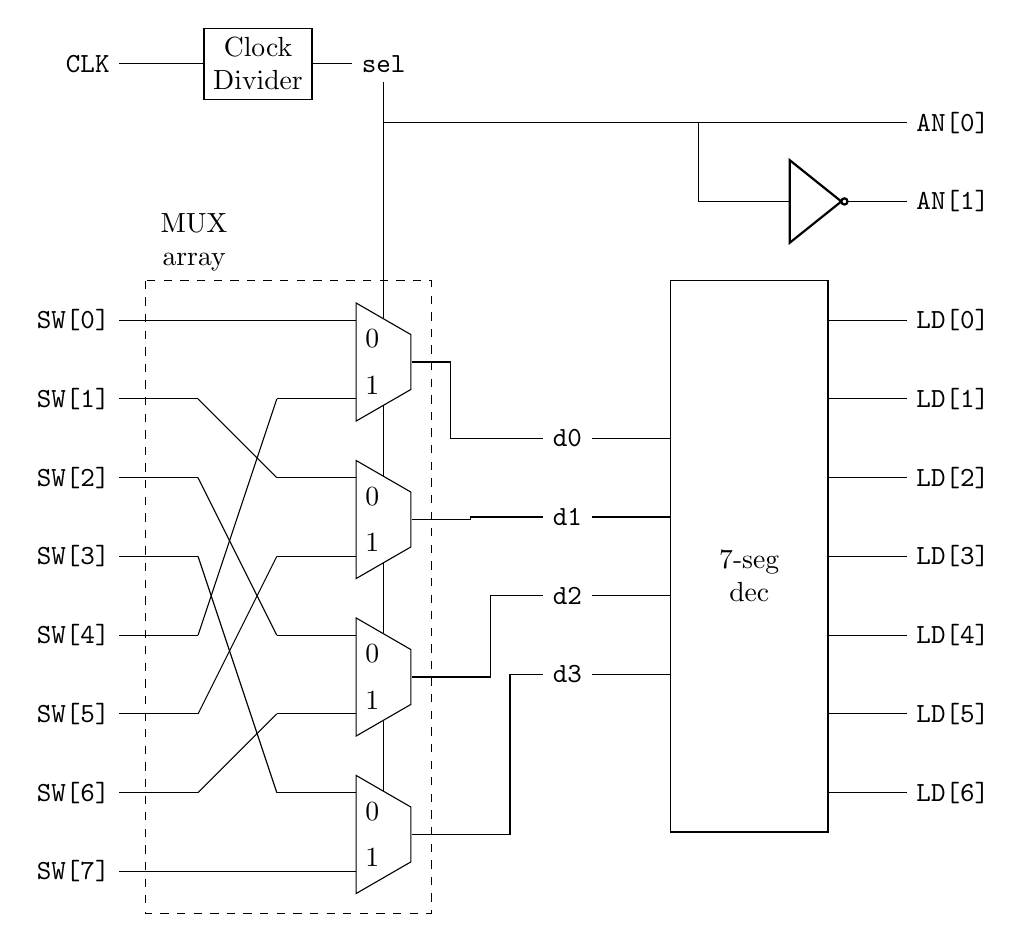
\begin{tikzpicture}
		\foreach \y in {0,1,...,6} {
			\draw (2,-\y) coordinate (o\y) -- ++(1,0) node[anchor=west] (ol\y) {\texttt{LD[\y]}};
		};
		\foreach \y in {0,1,2,3} {
			\draw ($(0,-1.5) + (0,-\y)$) coordinate (i\y) -- ++(-1,0) node[anchor=east] (dl\y) {\texttt{d\y}};
		};
		\foreach \y in {0,1,...,7} {
			\draw (-6,-\y) coordinate (s\y) -- ++(-1,0) node[anchor=east] (il\y) {\texttt{SW[\y]}};
			\draw (-4,-\y)-- ++(-1,0) coordinate (ms\y);
		};
		\foreach \y in {0,1,...,3} {
			\pgfmathtruncatemacro{\z}{2*\y}
			\pgfmathtruncatemacro{\a}{\y+4}
			\pgfmathtruncatemacro{\b}{\y*2+1}
			\draw (s\y) -- (ms\z);
			\draw (s\a) -- (ms\b);
		};
		\foreach \y in {0,2,...,6} {
			\node[anchor=north west,yshift=-5pt,multiplexer,scale=1.1,transform shape] at (-4,-\y) (m\y) {};
			\node[anchor=north west,yshift=5pt] at (m\y.north west) {0};
			\node[anchor=south west,yshift=-5pt] at (m\y.south west) {1};
		}
		\draw ($(o0)+(-2,0.5)$) rectangle ($(o6)+(0,-0.5)$);
		\node[align=center] at ($(i1)!0.5!(o4)$) {7-seg\\ dec};
		\node[anchor=south] at ($(m0.north)+(0,3)$) (sel) {\texttt{sel}};
		\draw (sel) -- (m0.north);
		\foreach \y in {0,2,4} {
			\pgfmathtruncatemacro{\b}{\y+2}
			\draw (m\y.south) -- (m\b.north);
		}
		\draw ($(sel)+(0,-0.75)$) coordinate (selbranch) to[*-] (selbranch -| ol0.west) node[anchor=west] {\texttt{AN[0]}};
		\draw ($(selbranch)+(4,0)$) to[*-] ++(0,-1) coordinate (selbranch2) -- ++(1,0) node[not port,anchor=in,scale=0.75,transform shape] (inv1) {} 
				(inv1.out) -- (selbranch2 -| ol0.west) node[anchor=west] {\texttt{AN[1]}};
		\draw (m0.east) -- ++(0.5,0) |- (dl0.west);
		\draw (m2.east) -- ++(0.75,0) |- (dl1.west);
		\draw (m4.east) -- ++(1,0) |- (dl2.west);
		\draw (m6.east) -- ++(1.25,0) |- (dl3.west);
		
		\node[rectangle,draw=black,anchor=east,align=center] at ($(sel.west)+(-0.5,0)$) (clkdiv) {Clock\\ Divider};
		\draw (sel.west) -- (clkdiv.east) (clkdiv.west) -- (clkdiv.west -| il0.east) node[anchor=east] {\texttt{CLK}};
		\draw[dashed] ($(il0.east)+(0.33,0.5)$) rectangle ($(m6.east)+(0.25,-1)$);
		\node[anchor=south west,align=center] at ($(il0.east)+(0.4,0.5)$) {MUX\\ array};
	\end{tikzpicture}
%\end{center}
\label{fig:7segDisplay}





To implement this design, we will create a 4-to-16 decoder and use it to make a new version of the seven-segment display decoder. We will use the clock divider to create the \texttt{sel} signal that selects between digit 0 and digit 1. We will create a \textbf{MUX array} module to switch between the inputs for digit 0 and digit 1, which will be taken from the top four switches and the bottom four switches, respectively. 

\subsection{4-to-16 Decoder Module}

For your first new module in this project, create a new Verilog source named \texttt{decoder4\_16.v}. This decoder will take a four-bit address input to assert one bit from a sixteen-bit output vector. Include an \texttt{en} input signal to enable your decoder. This module is going to be a \textbf{structural design}, meaning all internal signals are declared as \texttt{wire} type and we will not use any \texttt{always} block. Your design should implement the schematic you designed in pre-lab exercise 1. You will need to instantiate two \texttt{decoder3\_8} modules, and you will need to define the \texttt{en} signals for those modules. The solution is partially completed for you in the code below.

\begin{lstlisting}
	wire en1, en2;
	// Create an assign statement to define the logic for en1 and en2
	
	decoder3_8 low (
			.en(en1),
			.d(),  // <--- fill in the d inputs
			.o(o[7:0])
		);
	decoder3_8 high (
			.en(en2),
			.d(),  // <--- fill in the d inputs
			.o(o[15:8])
		);
\end{lstlisting}

% As before, simulate the design to verify it. \textbf{You don't need to program this one.}\\

% \textbf{ Note: } If you have inverted results check $en1$ and $en2$. \\

As before, simulate the design to verify it. \textbf{You don't need to program this one. Note that if you have inverted results, check $en1$ and $en2$.}

\textbf{Simulation Note:} When you have multiple testbenches, don't forget to set the testbench you want to run at the top module under simulation sources (this is separate from the design sources top module). When you launch simulation it will simulate which ever module is set as top. If you have a simulation window open and then change the top module, you must close the simulation window and then restart the simulation, else the changes will not take effect.
\begin{center}
	\includegraphics[height=5in]{images/sim_hierarchy.png}
\end{center}
\subsection{Parameterized MUX Array Module}

Your next module will be a flexible MUX array. Create a new source called \texttt{MUXarray.v} with the following I/O signals:
\begin{center}
\begin{tabular}{cccc}
direction & name & vector & bits \\
\hline
\texttt{input} & \texttt{a} & yes & 3:0 \\ 
\texttt{input} & \texttt{b} & yes & 3:0 \\ 
\texttt{input} & \texttt{sel} & no & -- \\ 
\texttt{output} & \texttt{o} & yes & 3:0 
\end{tabular}
\end{center}
In this module, we are going to create an array of four MUX modules so that we can switch between two four-bit vectors. In order to do this efficiently, we will make use of Verilog's \texttt{generate} syntax which allows us to declare a regular array of modules. A bonus from using this technique is that we can make a \textbf{reusable general-purpose MUX array} by using Verilog's \texttt{parameter} syntax. This will make our MUX array adaptable to any size of input vectors, and will be useful for saving work in future designs.

The flexible syntax is demonstrated in the module shown below. Since we need to have parameterized input and output vector sizes, the parameter declaration must come first, using the syntax 

\begin{lstlisting}
module <module_name> #(parameter <param_name>=<default_value>) (
	<port definitions>
);
\end{lstlisting}


Then we can use the parameter in a \texttt{generate} statement as shown below:

\begin{lstlisting}
module MUXarray #(parameter SIZE=4) (
	input sel,
	input [SIZE-1:0] a,
	input [SIZE-1:0] b,
	output [SIZE-1:0] o
);
	
	genvar i;
	
	generate 
		for (i=0; i<SIZE; i=i+1) begin: MUXarray 
			mux m(
				.i({a[i],b[i]}),
				.sel(sel),
				.o(o[i])
			);
		end
	endgenerate
	
endmodule
	
\end{lstlisting}

The \texttt{generate} array contains three essential elements: (1) a \texttt{genvar} variable to be used in the \texttt{for} loop; (2) the actual \texttt{generate/endgenerate} block; and (3) a named \texttt{for} loop initiated with \texttt{begin: <name>} and terminated with \texttt{end}. In our case the loop is named ``\texttt{MUXarray}'', which happens to be the same as the module name (but we could name the loop anything, excluding Verilog keywords, if we were feeling creative.) Anything you instantiate inside the \texttt{for} loop will be repeated \texttt{SIZE} times. This is an incredibly useful shorthand for building structural designs.

When instantiating the parameterized MUX array, whether in a testbench or in a hierarchical design, you can use the default parameter setting (4 in this case) by declaring the instance as usual. To set an alternative value of the parameter, you need to specify it using the \# syntax:
\begin{lstlisting}
   wire [3:0] a, b, o;
   wire [7:0] big_a, big_b, big_o;
   
   // Default parameter, size of 4:
   MUXarray             mux1(.sel(sel),.a(a),.b(b),.o(o));     
   
   // Modified parameter, size of 8:         
   MUXarray #(.SIZE(8)) mux2(.sel(sel),.a(big_a),.b(big_b),.o(big_o));  
   
\end{lstlisting}
In this design, it so happens we will only use the default size. In the future, however, you may need to reuse this \texttt{MUXarray} module for vectors with a different length.


\subsection{New Seven-Segment Decoder}
% Old wording - Nick removed the mention to pre-lab 6, as that is no longer a pre-lab exercise
%
% In pre-lab exercise 6, you were asked to implement a truth table by using a 3-to-8 decoder  with OR gates. In exercise 5 you were asked to convert the seven-segment truth table columns into hexadecimal. Now, in this lab step, you will combine those approaches to create a seven-segment decoder based on the 4-to-16 decoder module. Create a new Verilog module in your project called \texttt{NewSevenSegment.v}.

In exercise 3 of the pre-lab, you were asked to convert the seven-segment truth table columns to hexadecimal. In pre-lab exercise 5, you were asked to implement a truth table using a 3-to-8 decoder and OR gates. Now, in this lab step, you will combine these approaches to create a seven-segment decoder based on the 4-to-16 decoder module. 

To efficiently model a truth table in Verilog, we can take advantage of the fact that the decoder outputs a multi-bit vector in which all bits are zero except for the selected signal. Therefore, if we apply a \textbf{bit-wise AND} operation over the decoder's output, \texttt{d}, together with the truth table output, \texttt{f} (the hexadecimal you created from the truth table in the pre-lab), it will select precisely the desired row from the truth table. When the desired row is selected, the correct segments can be powered on the display for a given input value.

An example showing this method is given below. The example uses a 2-to-4 decoder instead of a 4-to-16 decoder. The example also uses \texttt{d} and \texttt{f} vectors that are 4-bits wide instead of 16-bits wide.

\begin{center}
	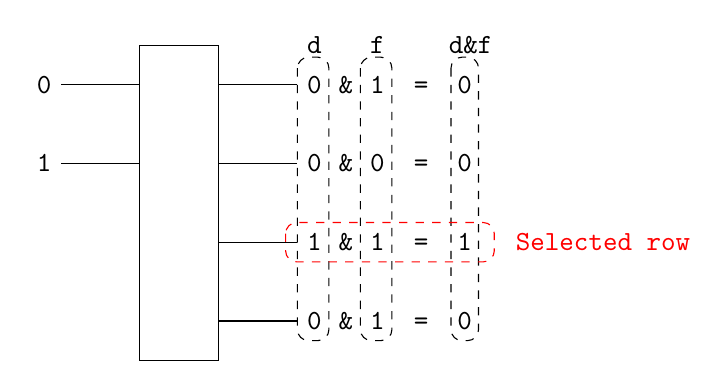
\begin{tikzpicture}
		\foreach \y in {0,1,2,3} {
			\draw (0,-\y) coordinate (d\y) -- ++(1,0) coordinate (dl\y);
			\node[anchor=west,xshift=0.4cm] at (dl\y) {\texttt{\&}};
		}
		\foreach \y in {0,1} {
			\draw (-1,-\y) coordinate (i\y) -- ++(-1,0) coordinate (il\y);
		}
		\draw ($(i0)+(0,0.5)$) rectangle ($(d3)+(0,-0.5)$);
		\node[anchor=east] at (il0) {\texttt{0}};
		\node[anchor=east] at (il1) {\texttt{1}};
		\node[anchor=west] at (dl0) {\texttt{0}};
		\node[anchor=west] at (dl1) {\texttt{0}};
		\node[anchor=west] at (dl2) {\texttt{1}};
		\node[anchor=west] at (dl3) {\texttt{0}};
		\node[anchor=west,xshift=0.8cm] at (dl0) {\texttt{1~~= ~0}};
		\node[anchor=west,xshift=0.8cm] at (dl1) {\texttt{0~~= ~0}};
		\node[anchor=west,xshift=0.8cm] at (dl2) {\texttt{1~~= ~1}};
		\node[anchor=west,xshift=0.8cm] at (dl3) {\texttt{1~~= ~0}};

		\node[anchor=west,xshift=0.8cm, yshift=0.5cm] at (dl0) {\texttt{f}};
		\draw[dashed,rounded corners] ($(dl0)+(0.8,0.35)$) rectangle ($(dl3)+(1.2,-0.25)$);
		\node[anchor=west, yshift=0.5cm] at (dl0) {\texttt{d}};
		\draw[dashed,rounded corners] ($(dl0)+(0,0.35)$) rectangle ($(dl3)+(0.4,-0.25)$);
		\node[anchor=west,xshift=1.8cm, yshift=0.5cm] at (dl0) {\texttt{d\&f}};
		\draw[dashed,rounded corners] ($(dl0)+(1.95,0.35)$) rectangle ($(dl3)+(2.3,-0.25)$);

        % highlight the selected row, added by nick to clarify this section
        \node[anchor=west, xshift=2.65cm,red] at (dl2) {\texttt{Selected row}};
        \draw[dashed,rounded corners,red] ($(dl2)+(-.15,0.25)$) rectangle ($(dl2)+(2.5,-0.25)$);

	\end{tikzpicture}
\end{center}

% Nick rewrote this section for clarity.
%
% The module code is partially completed below; you will need to fill in the missing entries based on your Pre-Lab exercises. \textbf{NOTE:} the result from the bit-wise AND operation of \texttt{d} and \texttt{f} is a 16-bit vector too, but we are assigning the result to a single bit in \texttt{seg[x]}. By default, Verilog will just assign this the lowest bit from the 16 bit result, we don't want this behavior. If any of the sixteen bits are HIGH we want the corresponding \texttt{seg[x]} to also be HIGH. We can achieve this by doing a reduction OR and is written in Verilog by having a leading $`\mid`$ with no operands on the left side. Here are some examples:
The result from the bit-wise AND, \texttt{d\&f}, is another 4-bit vector. This is because \texttt{d} and \texttt{f} are both 4-bit vectors. However, we just want to drive a one-bit scalar, \texttt{seg[x]}, to tell us whether or not each segment of the display should turn on. If we assign the signal like this:
\begin{lstlisting}
    assign seg[x] = d & f;
    // incorrectly assigning a multi-bit vector to a one bit scalar
\end{lstlisting}

We will be attempting to assign a multi-bit vector, \texttt{d\&f}, to a one bit scalar, \texttt{seg[x]}. By default, Verilog will just assign the lowest bit from \texttt{d\&f} to \texttt{seg[x]}, which is not the behavior that we want. This is how the Verilog compiler would, by default, interpret the previous code:
\begin{lstlisting}
    assign seg[x] = (d&f)[0];
    // By default, Verilog selects the lowest bit of the result
\end{lstlisting}

To fix this issue, we will perform a reduction OR on the multi-bit \texttt{d\&f}. The syntax for a reduction OR places a leading `\texttt{|}` with no operands on the left side.
\begin{lstlisting}
    wire [15:0] b;
    wire a;

    assign a = |b; // reduction OR of 16-bit vector b into a
    // a will equal `1' if one or more bits in b are `1'
\end{lstlisting}

The reduction OR operator ORs together each bit of a multi-bit vector and outputs the result as a one-bit scalar. The result is that the output of the operation is a `1' if at least one of the input bits is a `1'. Here are some 4-bit examples of the reduction OR operator:
 % updated with "equivalent to..." comments to clarify the behavior -Nick
\begin{lstlisting}
    | 4'b0000 = 0
        // equivalent to: 0 | 0 | 0 | 0 = 0
        
    | 4'b0101 = 1
        // equivalent to: 0 | 1 | 0 | 1 = 1
\end{lstlisting}

Create a new source file called NewSevenSegment.v. The module code is partially completed below. You will need to use the hexadecimal values from exercise 3 of the pre-lab and what you learned about the reduction OR operator to fill in the rest of the module.
\begin{lstlisting}
module NewSevenSegment(
    input [3:0] wxyz,
    output [6:0] seg //
    );

	wire [15:0] d;
	// NOTE: your port names may be different
	// depending on what you named them in the 4-16 decoder
	decoder4_16 D(.d(wxyz), .en(1), .o(d));

	assign seg[0] = // ENTER YOUR SOLUTION for a
	assign seg[1] = // ENTER YOUR SOLUTION for b
	assign seg[2] = // ENTER YOUR SOLUTION for c
	assign seg[3] = // ENTER YOUR SOLUTION for d
	assign seg[4] = // ENTER YOUR SOLUTION for e
	assign seg[5] = // ENTER YOUR SOLUTION for f
	assign seg[6] = // ENTER YOUR SOLUTION for g
endmodule
\end{lstlisting}

\textbf{Note:} Hexadecimal numbers in verilog are entered with the number of bits followed by 'h, then the hex number.

\begin{lstlisting}
    // Example: 8'hAB == 8'b10101011
    // Example: 6'hAB == 6'b101011
\end{lstlisting}

\textbf{Verifying your new seven-segment module:} Since you previously completed some alternative designs for the same seven-segment decoder function, you can check your new design against the old one. Specifically, you should copy the source for your \texttt{SevenSegmentTruthTable} module from Lab 2. Your new module should have exactly the same behavior as the old one. We can test their equivalence by creating instances of the new module and the old module, providing them both with the same input signals. If there is any error in your new module design, then at least one of its outputs will be different from \texttt{SevenSegmentTruthTable}. We can detect any difference by using XOR operations on the respective signals. So your test structure should look like this:
%\ctikzset{tripoles/american xor port/input skip=0.1}
%\ctikzset{tripoles/american xor port/input height=}
%\ctikzset{tripoles/american xor port/port width=}
\ctikzset{tripoles/american xor port/distance=0.25}
\ctikzset{tripoles/american xor port/aaa=0.5}
\ctikzset{tripoles/american xor port/bbb=0.2}
\ctikzset{tripoles/american xor port/ccc=0.8}
\ctikzset{tripoles/american xor port/ddd=0.2}
\begin{center}
	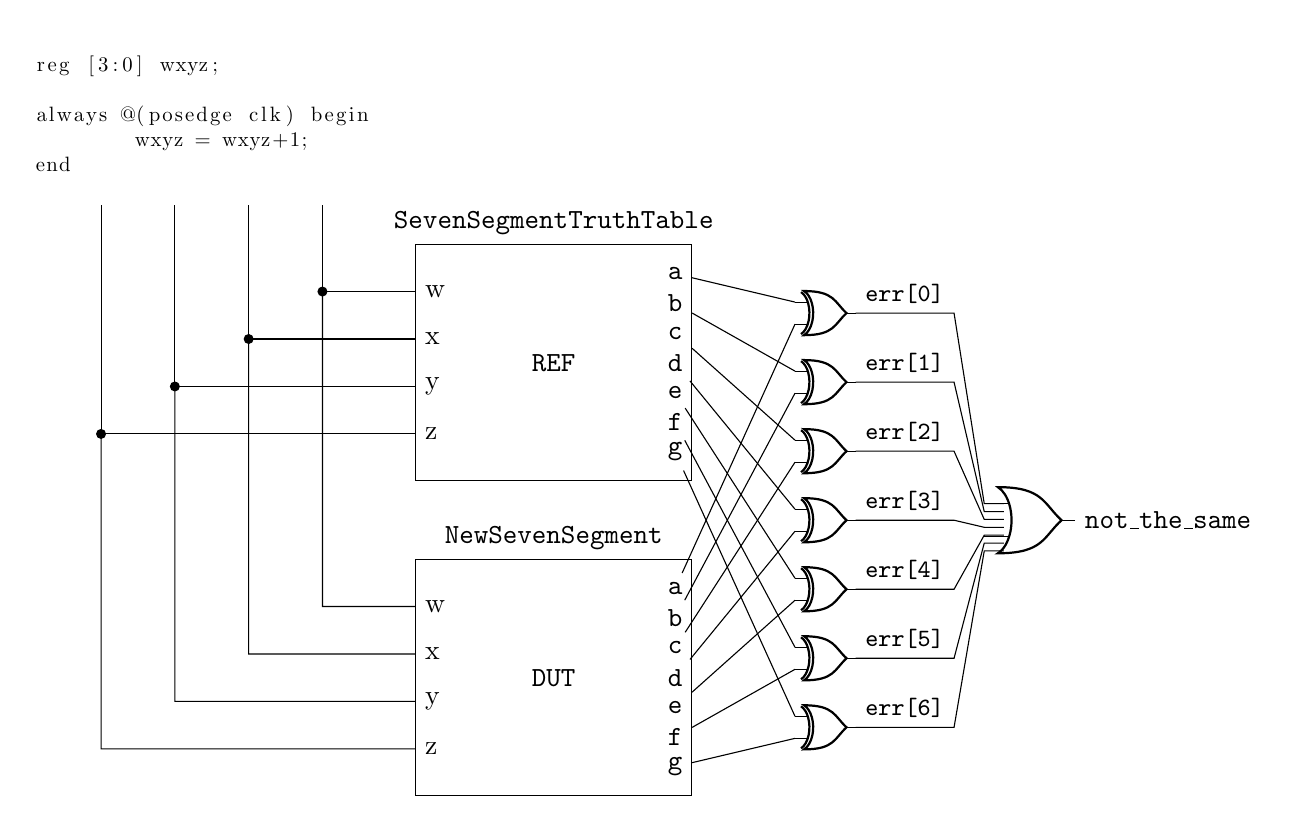
\begin{tikzpicture}
		\node[draw=black,minimum width=3.5cm,minimum height=3cm] at (0,0) (sstt) {\texttt{REF}};%SevenSegmentTruthTable}};
		\node[draw=black,minimum width=3.5cm,minimum height=3cm] at (0,-4) (nss) {\texttt{DUT}};%NewSevenSegment}};
		\node[anchor=south] at (sstt.north)  {\texttt{SevenSegmentTruthTable}};
		\node[anchor=south] at (nss.north)  {\texttt{NewSevenSegment}};
		\node[anchor=south east,minimum height=3cm,scale=0.75,transform shape] at (-2,2) (always) {\begin{minipage}{6cm}
		\begin{lstlisting}
reg [3:0] wxyz;

always @(posedge clk) begin
	wxyz = wxyz+1;
end
\end{lstlisting}
		\end{minipage}
		};
		\foreach \x/\y in {0/w,1/x,2/y,3/z} {
			\pgfmathparse{(1.0+\x)/5.0}
			\node[anchor=west] at ($(sstt.north west)!\pgfmathresult!(sstt.south west)$) (ssttin\x) {\y};		
			\draw ($(always.south east)!\pgfmathresult!(always.south west)$) coordinate (\y) -- (\y |- ssttin\x.west) coordinate (j\y) -- (ssttin\x.west);
			};
		\foreach \x/\y in {0/a,1/b,2/c,3/d,4/e,5/f,6/g} {
			\pgfmathparse{(1.0+\x)/8.0}
			\node[anchor=east] at ($(sstt.north east)!\pgfmathresult!(sstt.south east)$) (ssttout\x) {\texttt{\y}};		
	
			};
		\foreach \x/\y in {0/w,1/x,2/y,3/z} {
			\pgfmathparse{(1.0+\x)/5.0}
			\node[anchor=west] at ($(nss.north west)!\pgfmathresult!(nss.south west)$) (nssin\x) {\y};		
					\draw (j\y) to[short,*-]  (j\y  |- nssin\x.west) -- (nssin\x.west); 
			};
		\foreach \x/\y in {0/a,1/b,2/c,3/d,4/e,5/f,6/g} {
			\pgfmathparse{(1.0+\x)/8.0}
			\node[anchor=east] at ($(nss.north east)!\pgfmathresult!(nss.south east)$) (nssout\x) {\texttt{\y}};		
			};
		\coordinate (a) at ($(sstt.north east)+(2,0)$);
		\coordinate (b) at ($(nss.south east)+(2,0)$);
		\node[or port,scale=0.75,transform shape] at ($(a)!0.5!(b)+(2.75,0)$) (or1) {};
		\foreach \x in {0,1,...,6} {
			\pgfmathparse{(1.0+\x)/8.0}
			\node[xor port,scale=0.5] at ($(a)!\pgfmathresult!(b)$) (xor\x) {};
			\pgfmathparse{(0.0+\x)/6.0}
			\draw (ssttout\x) -- (xor\x.in 1) (nssout\x) -- (xor\x.in 2) (xor\x.out) -- ++(1.25,0) -- ($(or1.in 1)+0.1*(0,-\x)$) -- ++(0.25,0) ;
			\node[anchor=south west] at (xor\x.out) (xl\x) {\small \texttt{err[\x]}};
		};
			\node[anchor=west] at (or1.out) (ol) {\texttt{not\_the\_same}};
	\end{tikzpicture}
\end{center}

This verification is simpler than it appears. Follow these steps:
\begin{itemize}
\item First, modify your copy of \texttt{SevenSegmentTruthTable.v} so that its inputs and outputs are vectors, just like the I/O ports used in \texttt{NewSevenSegment.v}. 
\item Then create a \texttt{Verilog Testbench} using the \texttt{New Source} wizard and associate it with \texttt{NewSevenSegment.v}. 
\item Modify your testbench to create a clock source, and create a four-bit \texttt{reg} signal named \texttt{wxyz}, initialized to zero. Then create three seven-bit \texttt{wire} signals named \texttt{segNew} and \texttt{segTruthTable} and \texttt{err}.  Lastly create a single-bit \texttt{wire} signal named \texttt{not\_the\_same}.
\item In the \texttt{DUT} instance statement, set the input to \texttt{wxyz} and the output to \texttt{segNew}.
\item Copy and paste the instance declaration for your \texttt{DUT} module, which should be of type \texttt{NewSevenSegment}. In the pasted line, change the module type to \texttt{SevenSegmentTruthTable} and the instance name to \texttt{REF} (for ``reference design''). Set \texttt{REF}'s input to \texttt{wxyz} and its output to \texttt{segTruthTable}.
\item Now create an \texttt{assign} statement to set \texttt{err = segNew$^\wedge$segTruthTable}. This will compute the \textbf{bit-wise XOR operation} over all respective bits in the two vectors.
\item Create another \texttt{assign} statement to set \texttt{not\_the\_same = |err}. This will compute the \textbf{reduction OR operation} over all the elements in \texttt{err}, reducing it to a single bit.
\item Lastly, create an \texttt{always} block, sensitive to \texttt{posedge clk}, which increments \texttt{wxyz} through all of its binary values.
\end{itemize} 

Now, when you simulate the design, you should see \texttt{wxyz} count through values from 0 up to 15, then roll over back to 0 and up to 15 again. Through all of this, you should see a lot of activity in \texttt{segNew} and \texttt{segTruthTable}, but the error signal \texttt{not\_the\_same} should stay flat at zero. If it stays at zero, this tells you the two modules are behaving exactly the same. The correct result should look like this:

\begin{center}
	\includegraphics[width=0.74\textwidth]{images/ReferenceComparison.png}
\end{center}
Notice that \texttt{not\_the\_same} stays flat through the whole simulation. It detects no discrepancies between my two module designs.

\textbf{NOTE:} it's easy to deceive yourself by computing incorrect expressions. For example, if you XOR \texttt{segNew} with itself, the result will be forever zero. If you inadvertently assign \texttt{not\_the\_same} to zero, then obviously it will stay at zero. Make sure your assign statements are computing the right calculation before you declare victory.

\textbf{Second NOTE:} If you see a lot of errors, it {\em could be} due to one of your modules having reverse-order port signals. Study your module outputs and check if they are appearing in reverse order. If, for example, \texttt{segNew[0]} is identical to \texttt{segTruthTable[6]}, then one of your modules is wired backwards, and you need to modify it to reverse the order of signals in the output vector. Or, you may have one output as the inverse of the other module, depending on where you inverted the 7 segment signal from lab 2.


\subsection{Multi-Digit Seven-Segment Display}
Now create a file called \texttt{DoubleSevenSegment.v}, and create submodule instances to implement a structural description of the top-level design. You will use the \texttt{MUXarray}, the \texttt{NewSevenSegment} and the \texttt{clockdivider} modules. Don't forget to invert the output of the NewSevenSegment module like you did in lab 2, by doing something like "assign seg = $\sim$D".
\\
Next, enter in the divider ratio as a parameter like so
\begin{lstlisting}
module DoubleSevenSegment #(parameter PRESCALER = 8)(// <-- replace '8'
// with your calculated value from the prelab
    input clk,
    // add the other needed inputs and outputs here

    );

	wire sel;
	
	ClockDivider  #(.PRESCALER(PRESCALER)) CKD( 
			.clkin(clk),
			.clkout(sel)
		);
	
	// add other signals and modules here
endmodule
\end{lstlisting}
 Use the value that you calculated in the pre-lab to achieve a \SI{.5}{\milli\second} positive phase for the clock (i.e.\ the total clock period should be \SI{1}{\milli\second}). Then customize an XDC constraint file to assign the board I/O signals as shown in the top-level design. Refer back to the block diagram at the beginning of this section if needed.

To verify your design, create a Verilog testbench and create the appropriate test signals. Try to rigorously study and interpret the simulation traces to make sure your design does what is intended. In the testbench, it's best to pass in a smaller PRESCALER value like 8, that way you don't have to wait thousands of clock cycles to see the anode switch in simulation.
\begin{lstlisting}
DoubleSevenSegment #(.PRESCALER(8)) DUT(
// add your ports here
    );
\end{lstlisting}
Then implement the design and program your board. You should see two illuminated digits on the seven segment display. You can change one digit by altering the top four switches, and the other digit is set by the bottom four switches. For each digit, enter all binary values from 0 to 15. The displays should show corresponding hexadecimal values for values above 9.

\subsection{Hints:}
    $1:$ Make sure to set any unused anodes to $1$. This is because anodes are active low so setting them to $1$ turns them off. \\
    $2:$ Make sure that you calculate your hexadecimal values from the pre-lab based on using the \textit{NAN} truth table from lab $2$. The \textit{NAN} table is the one that doesn't display the numbers $10 - 15$.
\section{TA Checkoff}

\begin{itemize}
\item (24 points) Complete pre-lab work prior to start of the lab.
\item (12 points) Correct design, simulation and demonstration of the 3-to-8 decoder module.
\item (12 points) Correct design, simulation and demonstration of the 2-to-1 MUX module.
\item (12 points) Correct design and simulation of the 4-to-16 decoder module.
\item (12 points) Correct design and simulation of the parameterized array MUX module.
\item (18 points) Correct design and simulation of the seven-segment decoder module.
\item (20 points) Correct design, simulation and demonstration of the Top-Level Design for the Multi-Digit Seven-Segment Display.
\end{itemize}

\end{document}